
\newpage
\section{Evaluation}
Below we present our evaluation process, that place the prototype in the hands of real people, as recommended by validated guidelines \cite{article_mhealth, how_to_evaluate_tech_for_behaviour_change}.

Many people agree about the importance of designing systems for health and behaviour
change~\cite{article_mhealth, article_designing_for_healthy_lifestyles, article_designing_for_health_behaviour_change_hci}.
But each have varying opinions about how to evaluate these systems. Klasnja et al.~\cite{article_evaluate_tech_health_behaviour_change} focuses on system usability and does it meet the needs of users.
Whereas, Stawarz and Cox~\cite{article_designing_for_health_behaviour_change_hci} argue evaluating a system of this type requires information from other fields
to properly consider the systems effectiveness. The validated Behaviour Change Wheel Framework~\cite{article_behaviour_change_wheel} does just this.
Evaluating the system with validated behaviour change techniques from multiple domains. This project will use this framework to evaluate the chatbot with evaluation trials.
These will test the long-term effect and efficiency of the bot, with information from two fields of study, HCI and health psychology.

Evaluation trials are the final part of the Behaviour Change Wheel Framework~\cite{article_behaviour_change_wheel}.
HCI research that focuses on health interventions~\cite{article_mhealth}, demonstrates the importance of evaluation trials for evaluating mobile health systems.
These trials have three goals to test: objective-quantitative efficacy, subjective-qualitative feedback measures and real-world feedback about how the system is
utilised~\cite{article_evaluate_tech_health_behaviour_change}. I will conduct an evaluation trial for this project.\newline
\newline
The length of the trial will be based on two factors, the time needed to form a habit~\cite{article_how_habits_formed_modelling_habit_formation} and the results of a previous
habit formation trial~\cite{article_beyond_self_tracking_designing_apps}.
First, the number of repetitive days required for an action to be considered a habit varies based on the complexity of the action~\cite{article_how_habits_formed_modelling_habit_formation}.
Simple actions, such as drinking 2 glasses of water a day, can take a minimum of 18 days to form.
The suggested actions used for this project will be considered as simple, e.g. stretching for 30 seconds.
Second, a previous evaluation trial on habit-formation systems~\cite{article_how_habits_formed_modelling_habit_formation} showed an increase in habit automaticity after 4 weeks.
This project will mirror that timeframe.\newline
\newline
A 4-week evaluation trial will test the success of the chatbot by evaluating the tool and the effectiveness of each modality on users habit strength.
Chatbot interaction will be removed during the follow up study to test if users continue with the habit.
Participants will split into four groups, all groups will receive reminders, three groups will receive rewards each from a different modality,
and one group (control group) will not recieve any rewards.

Habit strength will be measured using a validated 12-question questionnaire that specifically looks at automaticity~\cite{article_habit_strength}.
Automaticity will also be measured using a validated subset of the questionnaire from~\cite{article_habit_strength} to test users habit behavioural
automaticity index~\cite{article_4q_SRBAI}. This will show the impact each modality has on habit automaticity and test the hypothesis.
Participants will fill out the questionnaires~\cite{article_habit_strength, article_4q_SRBAI} at three stages: half-way through the trial (at 2-weeks),
after the trial has finished and after the follow up trial.

\subsection{Study: Comparing Different Rewards} \label{study_comparing_rewards}
To explore the influence of different modalities on habit formation, a situated study was conducted, followed by semi-structured interviews. For the purpose of the study a chatbot was developed to help users form healthy habits by providing different types of positive reinforcement. The study and the bot itself are described below.


\subsubsection*{Hypotheses}
The study tests the two hypotheses (Section~\ref{hypothese}), H1: The rewards affect on habit performance and automaticity and H2: Multiple modes versus singular affect on habit performance and automaticity. They are measured by habit performance (measurement 1, M1), calculated by the number of habits a participant marked as completed, incremented when a participant presses '\textit{completed habit}' on the bot and habit automaticity  (measurement 2, M2), calculated from two Self-Report Behavioural Automaticity Index~\cite{article_4q_SRBAI} questionnaires. In addition to these two hypotheses, the success of the prototype is also evaluated during the interview stage.

\begin{figure}[H]
  \centering
  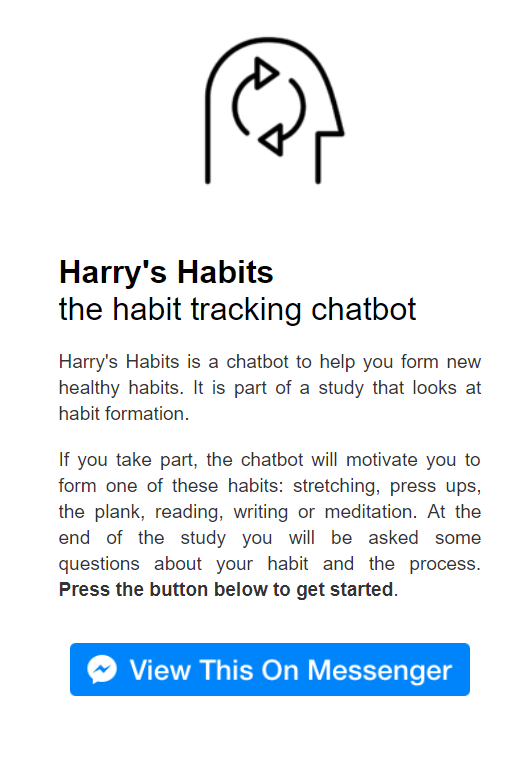
\includegraphics[width=2in]{resources/design/process/harryshabits-landing-page.png}
  \caption{The landing page (\url{www.harrymt.com/harryshabits}) participants would see before they are taken to the Messenger bot.}
  \label{fig:landing_page}
\end{figure}

\subsubsection{Method}
The study aims to test the hypotheses comparing how well people form new habits based on the rewards and how the bot-delivered rewards affect participants habit formation.

\begin{figure}[H]
  \centering
  \begin{tabular}{l l l}
    {\small\textit{Modality}} & {\small \textit{Reward}} & {\small \textit{No. Participants}}  \\ \hline
    visual & 15s gif & 15 \\
    auditory & 15s audio & 15 \\
    visual-auditory & 15s gif and audio & 15 \\
    none (control group) & no reward & 15 \\
  \end{tabular}
  \caption{Participants were randomly assigned one of these four rewards.}~\label{fig:precise_rewards}
\end{figure}

\subsubsection{Participants}
60 participants were recruited on social networks (using the landing page: \url{www.harrymt.com/harryshabits}), and were mostly University students and staff. The process participants undertook is documented by the recruitment adverts (Appendix~\ref{app:recruitment}), the landing page (Figure~\ref{fig:landing_page}) and the setup screens (Section~\ref{user_flow}). They were instructed to connect with the bot via Facebook Messenger and pick a series of options to set-up their habit tracking. Participants answered general demographic information as set up questions from the bot when they connected with it (Section~\ref{user_flow}).

\begin{itemize}
  \item ``What is your gender?''
    \item ``How old are you?''
    \item ``Have you used habit tracking systems before? If did they work and what were they?''
    \item ``What habit do you want to track?''
    \item ``What existing routine would you like to use?''
    \item ``What time does that routine occur?''
    \item ``Would you like to be interviewed about your experience after the study?''
\end{itemize}


\subsubsection{Design}
A brief description accompanied these questions, to guide the participants on how to answer. The habits participants could choose were split into two categories, physical and relaxation. They were: stretching, press ups, the plank, reading, writing or meditation.
The study used four conditions: visual rewards, auditory rewards, visual-auditory rewards and no rewards (control group). Participants were randomly assigned a condition by the bot after they completed the set-up, 15 were assigned to visual rewards, 15 assigned to auditory rewards, 15 assigned to visual-auditory rewards and 15 with no rewards (control group).
Participants would receive a confirmation message, followed by a positive reinforcement reward after they marked a habit as complete, unless they were in the control group, then they would only receive a confirmation message.

\begin{figure}[H]
  \centering
  \begin{enumerate}
    \item ``[Habit] after [context] is something I do automatically.''
    \item ``[Habit] after [context] is something I do without having to consciously remember.''
    \item ``[Habit] after [context] is something I do without thinking.''
    \item ``[Habit] after [context]  is something I start doing before I realise I am doing it.''
  \end{enumerate}
  \caption{SRBAI questionnaire~\cite{article_4q_SRBAI} to measure habit automaticity, presented at the end of week 3 and week 4 during the study for Harry's Habits.}
  \label{fig:srbai_questionnaire}
\end{figure}

\subsubsection{Materials}
The bot will collect the amount of habits participants complete versus their reward type. Habit completion will be verified by using the SRBAI questionnaire~\cite{article_4q_SRBAI}---A validated set of questions to measure habit automaticity levels. This will be used to test if participants are forming a habit. Various questions about how participants found their rewards were also asked (Figure~\ref{fig:srbai_questionnaire}). Participants results will be stored in a password protected secure database. Finally, interviews with participants discuss the bot-delivered rewards for further verification.


\begin{itemize}
\item \textit{visual rewards}: participants would receive a message that when tapped, would reveal a gif aimed at motivating them.
\item \textit{auditory rewards}: participants would receive a message that when tapped, would play a song aimed at motivating them.
\item \textit{visual-auditory rewards}: participants would receive a message that when tapped, would play a song and reveal a gif, aimed at motivating them.
\item \textit{no rewards (control group)}: participants would only receive a confirmation message.
\end{itemize}

\subsubsection{Procedure}
First, a internal pilot trial was conducted to develop the strength of the prototype. Second, a  4-week situated trial was conducted with real people who wanted to try and form a new positive habit. Finally, follow-up interviews with participants revealed if participants continued with their habit without the bot.

The 4-week evaluation trial was split into two sections. First a 3-week trial tests the success of the chatbot by evaluating the tool and the effectiveness of each modality on participants habit automaticity using a validated questionnaire~\cite{article_4q_SRBAI}. During the fourth week, chatbot interaction is removed during a 1-week follow up trial to test if participants continue with the habit. Participants were split into four groups, all groups receiving reminders, three groups receiving rewards each from a different modality, and one group (control group) did not receive any rewards.

At the beginning of the 3-week period, participants were asked to answer basic demographic information and choose a new habit they would like to develop from a list of habits of similar difficulty, divided into two categories: physical and relaxation. Then they were asked to state an existing routine they could build their new habit around, and choose a time that routine normally occurred (Morning, Afternoon, Evening). After they had answered these questions, they would be randomly assigned a modality (unknowingly to users) for rewards. Participants would complete their chosen habit every day after their existing routine, then wait for the bot to send them a message asking them for one of two choices.

Option one (completed habit): participants would receive a message thanking them, then participants not in the control group would receive a message linking them to a reward. This reward would be from the modality auto-assigned to that participant during the set-up phase (Figure~\ref{fig:precise_rewards}). Option two (not yet): the bot would check on the participant an hour later. This allowed for the checks to be snoozed, to ensure the new habit fit in with participants routine. If participants constantly told the bot they hadn't completed their habit yet, the bot would ask participants if they would like to change the time their routine occurred (Figure~\ref{fig:snoozing_too_much}. This allowed the participants in the beginning to refine the time they would perform their habit.

\begin{figure}[H]
  \centering
  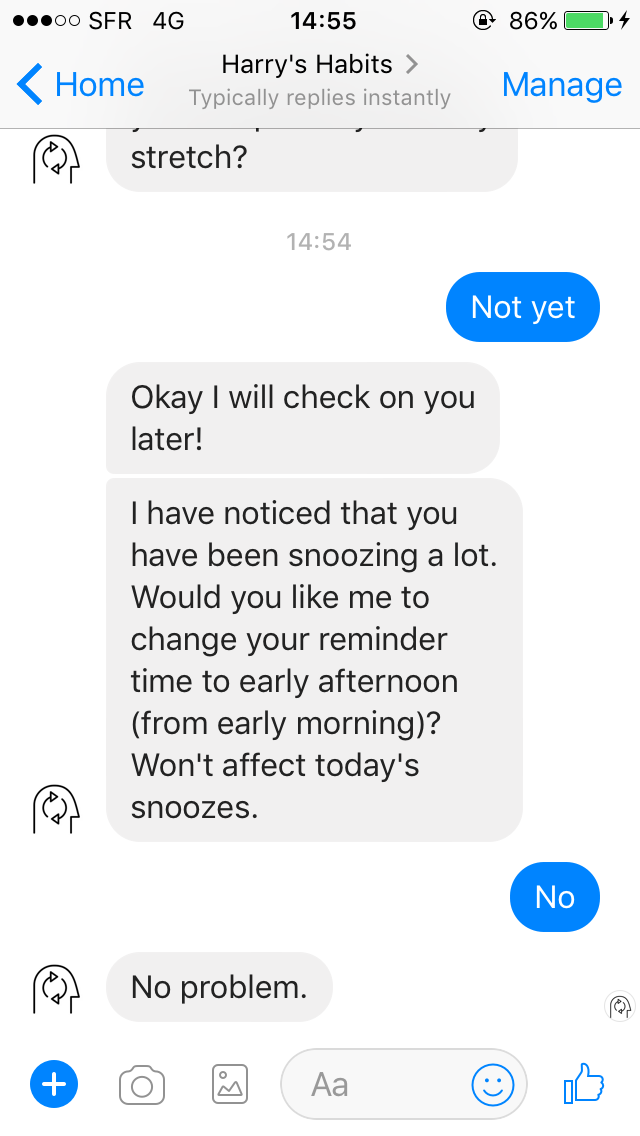
\includegraphics[width=2in]{resources/design/media/4.png}
  \caption{Participants would receive a message asking them if they would like to change their backup notification time.}
  \label{fig:snoozing_too_much}
\end{figure}

After 3 weeks of participants interacting with the bot, all participants who completed the set up are asked to complete the SRBAI questionnaire. Then the bot interaction was suspended for 1 week. After the full 4-week period, participants were asked to complete the questionnaire again. Both questionnaires presented the questions on a 5-point Likert scale with answers from 'Strongly Disagree' (5) to 'Strongly Agree' (1). Higher scores indicates higher self-reported levels of automaticity. In addition, participants had an option to opt-in for an interview about their experience after the 4-week period.

\subsection{Results}
60 participants connected with the bot by pressing \textit{'Get Started'} in Facebook Messenger on the following platforms: 25 browser, iOS 18 and Android 12. 14 participants (23\%) dropped out of the study at various stages (Figure~\ref{fig:study_dropout}): 54 participants (90\%) continued interacting with the bot and started the set-up. 39 participants (65\%) completed the set-up and out of these 39 participants, 3 participants just ignored all messages from the bot during the trial. Leaving 36 participants (66\%) that are considered active throughout and included in the final analysis. These 36 participants are 18-63 years old, (mean: 27 years old, SD: 12), 23 (64\%) male, 11 (30\%) female and 2 (6\%) didn't say. These 36 remaining participants are split into the following modalities: 14 participants (93\%) visual, 9 participants (60\%) visual-auditory, 7 participants (46\%) auditory and 6 participants (40\%) had no rewards (control group). 28 participants volunteered for an interview and 7 were carried out.

\begin{figure}[H]
  \centering
  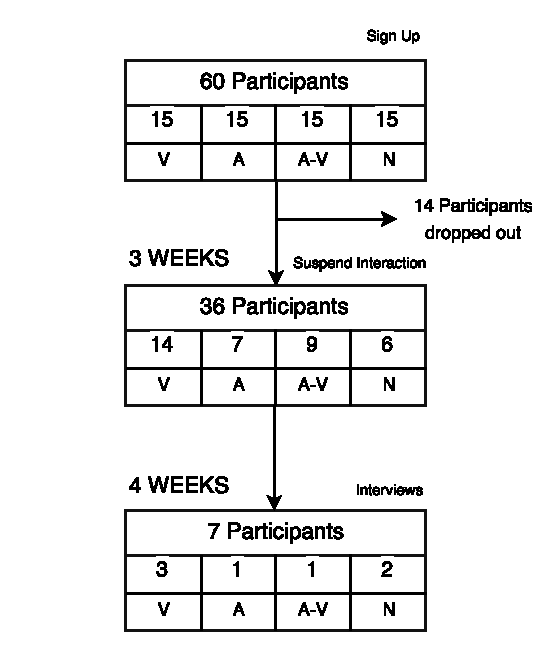
\includegraphics[width=.4\columnwidth]{resources/figures/study-flow.pdf}
  \caption{Participant drop-out during the 4-week study.}~\label{fig:study_dropout}
\end{figure}

36 participants sent a total of 1.1k messages to the bot (mean = 65 messages per participant). The bot sent 2.7k total messages back and made 2,995 calls to the Facebook API including 319 retry errors. 184 total habits were marked as completed, with the bot issuing 69 visual rewards, 58 visual-auditory rewards and 17 auditory rewards to those participants. The control group completed 40 habits and were sent 0 rewards.

Comparing the number of participants who dropped out of the study versus their reward modality, shows that 7 participants who blocked the bot had 27 visual rewards in total (mean = 3.85). 2 participants had 4 total auditory rewards (mean = 2) and 2 participants had 2 visual-auditory combined (mean = 6.5). These visual-auditory participants that dropped out had the highest amount of snoozes (24 total snoozes, 6 and 18 individually, mean = 12), compared with visual 10 total (mean = 2), and auditory with 0 snoozes.

7 participants (19\%) previously used habit tracking systems and 100\% of stated they worked well for tracking habits. These habits were: 'Diet' (3 mentions), 'Exercise' (3 mentions), 'Deadlines' (2 mentions), 'Audiobook reading' (1 mention), 'Weight' (1 mention). All of these participants chose new habits that they hadn't tracked before. Meditation was the most popular habit chosen (12 participants 33\%), followed by Press ups (8 participants 22\%), then Stretching (6 participants 15\%). Reading and writing were the least, only selected by 4 and 2 participants respectively. Stretching (6 participants 15\%) was the most completed habit based on selection (60 times), ranking 10.0 (where 10.0 = 60/6). Meditation ranked 6.25 (6.25 = 75/12) and the least were the plank and reading with 3.75 (15/4) and 1.75 (7/4) respectively.

Participants (14 participants 39\%) with visual rewards had the highest total number of snoozes (72 total presses to 'Not Yet'), auditory had the smallest (14 total). The control group had 55 snoozes and visual-auditory had 45 snoozes. Most participants snoozed (answered 'Not Yet') in the morning (100 times), specifically mid (66) and late (27) morning. Visual and sound had the most number of failed snoozes (10, split over 6 participants, 1 person had 5 failed snoozes). Then it was sound by 4.

Habit performance was also tracked in the form of a streak. If a participant did not track a habit for a day, their streak would be reset to 0. Meditation had the most cumulative streak (17) followed by stretching (7 participants). High streaks (streak > 10) had habits: meditation (total 135 streaks) and stretch (126 streaks). Visual-Auditory rewards had the most streaks (126 combined), control group had 75, then Visual had 60. Stretch had the highest peak streak (18), meditation (15). However, overall, for all habits completed, meditation was the most streaked (269 combined), stretching (231 combined), then press ups (39) then plank (24).

31 participants (86\%) chose a context that was listed as an example (Figure~\ref{fig:habit_context_example}), some had a slight change of wording e.g. before getting home from work, rather than after getting home from work. The remaining 5 people chose the following context: 'Having a snack', 'Sitting in bed', 'Early morning', 'during breakfast' and 'Before sleeping'.

\begin{figure}[H]
  \centering
  \begin{itemize}
    \item Morning
    \begin{itemize}
      \item waking up
      \item eating breakfast
      \item arriving at work
    \end{itemize}
    \item Afternoon
    \begin{itemize}
      \item eating lunch
      \item leaving work
    \end{itemize}
    \item Evening
    \begin{itemize}
      \item leaving work
      \item eating dinner
      \item getting ready for bed
    \end{itemize}
  \end{itemize}
  \caption{The examples given to participants for habit contexts based on the time they chose.}
  \label{fig:habit_context_example}
\end{figure}

\subsubsection*{M1: Habit Performance}
\begin{figure}[H]
\centering
 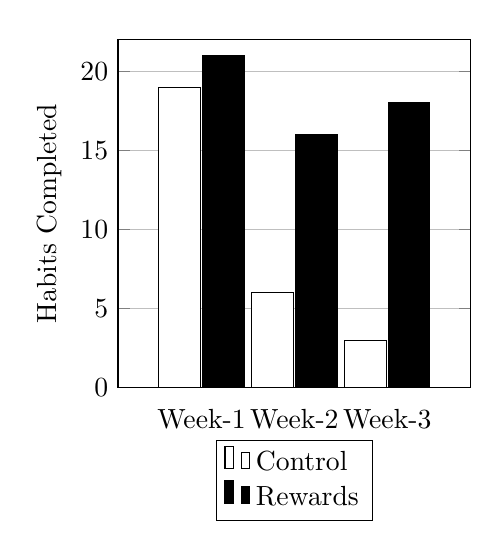
\begin{tikzpicture}
   \begin{axis}[
      width  = 0.5*\textwidth,
      height = 6cm,
      major x tick style = transparent,
      ybar=2*\pgflinewidth,
      bar width=15pt,
      ymajorgrids = true,
      symbolic x coords={Week-1, Week-2, Week-3},
      xtick = data,
      scaled y ticks = false,
      enlarge x limits=0.45,
      ymin=0,
      ymax=22,
      legend cell align=left,
      legend style={at={(0.5,-0.15)},anchor=north},
      ylabel={Habits Completed},
   ]
      \addplot[style={fill=white},error bars/.cd, y dir=both, y explicit]
          coordinates { % Control group
          (Week-1, 19)
          (Week-2, 6)
          (Week-3, 3)
          };

      \addplot[style={fill=black},error bars/.cd, y dir=both, y explicit,error bar style=red]
           coordinates { % Rewards
          (Week-1, 21)
          (Week-2, 16)
          (Week-3, 18)
           };

      \legend{Control, Rewards}

  \end{axis}
  \end{tikzpicture}
  \caption{H1M1: The rewards affect on habit performance. The sum of habits completed by participants with rewards versus the control group during 3-week study period.}~\label{fig:m1_h1}

 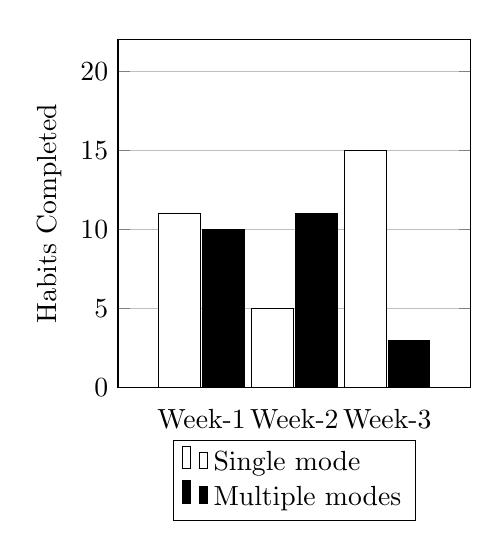
\begin{tikzpicture}
   \begin{axis}[
      width  = 0.5*\textwidth,
      height = 6cm,
      major x tick style = transparent,
      ybar=2*\pgflinewidth,
      bar width=15pt,
      ymajorgrids = true,
      symbolic x coords={Week-1, Week-2, Week-3},
      xtick = data,
      scaled y ticks = false,
      enlarge x limits=0.45,
      ymin=0,
      ymax=22,
      legend cell align=left,
      legend style={at={(0.5,-0.15)},anchor=north},
      ylabel={Habits Completed},
   ]

      \addplot[style={fill=white},error bars/.cd, y dir=both, y explicit,error bar style=red]
           coordinates { % Singular Modes
          (Week-1, 11)
          (Week-2, 5)
          (Week-3, 15)
           };
      \addplot[style={fill=black},error bars/.cd, y dir=both, y explicit]
          coordinates { % Multiple Modes
          (Week-1, 10)
          (Week-2, 11)
          (Week-3, 3)
          };

      \legend{Single mode, Multiple modes}

  \end{axis}
  \end{tikzpicture}

  \caption{H2M1: Multiple modes versus singular on habit performance. Sum of completed habits for multiple modalities compared with singular modes.}~\label{fig:m1_h2}
\end{figure}


\subsubsection*{H1M1: The rewards affect on habit performance}

A one-way between-groups analysis of variance with planned comparisons was conducted to explore the effect of rewards on the number of habits completed, compared with the control group (Figure~\ref{fig:m1_h1}). Participants were divided into two groups according to their reward mode (Group 1: visual rewards, auditory rewards, visual-auditory rewards; Group 2: control group). There was a statistically significant difference at the p \verb|<| .005 level in both groups for 2\/3 of the Weeks: Week 1, F (1, 23.20) = 9.48, p = .005, Week 2, F (1, 33.35) = 4.46, p = 0.42 and Week 3, F (1, 50) = 17.01, p \verb|<| 0.005. The effect size for Week 1, Week 2 and Week 3 are large, calculated using eta squared, were 0.25, 0.39 and 0.43 respectively, this shows a large difference in the mean scores.


\subsubsection*{H2M1: multiple modalities versus singular mode}
A one-way between-groups analysis of variance with planned comparisons was conducted to explore the effect of multiple modalities and singular modalities on the number of habits completed (Figure~\ref{fig:m1_h2}). Participants were divided into two groups according to their mode (Group 1: visual rewards, auditory rewards; Group 2: visual-auditory rewards). There was a statistically significant difference at the p \verb|<| .005 level in Week 2 and Week 3, and lots in all groups: Week 1, F (1, 50) = 0.69, p = .410, Week 2, F (1, 50) = 23.04, p \verb|<| .005 and Week 3, F (1, 50) = 8.85, p = .005. The effect size for Week 1, Week 2 and Week 3 are large, calculated using eta squared, were 0.25, 0.39 and 0.43 respectively, this shows a large difference in the mean scores.





\subsubsection*{M2: Habit Automaticity}
11 participants completed both SRBAI questionnaires, 2 control group, 2 auditory, 5 visual and 2 visual-auditory. A paired-samples t-test was conducted to evaluate the change of habit automaticity between the first SRBAI questionnaire (after week 3) and the second (after week 4). There was a statistically significant increase in automaticity scores from SRBAI 1 (mean = 14.18, SD = 3.78) to SRBAI 2 (mean = 15.09, SD = 4.34), t (10) = 2.469, p \verb|<| .005 (two-tailed). The mean increase in SRBAI scores was 0.90 with a 95\% confidence interval ranging from 0.08 to 1.72. The eta squared statistic (.37) indicated a large effect size.


%       S1 Mean S2 Mean S1 SD   S2 SD
% Control 13.5  14.5  4.949747468 6.363961031
% Rewards 14.33 15.22 3.840572874 4.294699576

\begin{figure}[H]
  \centering
 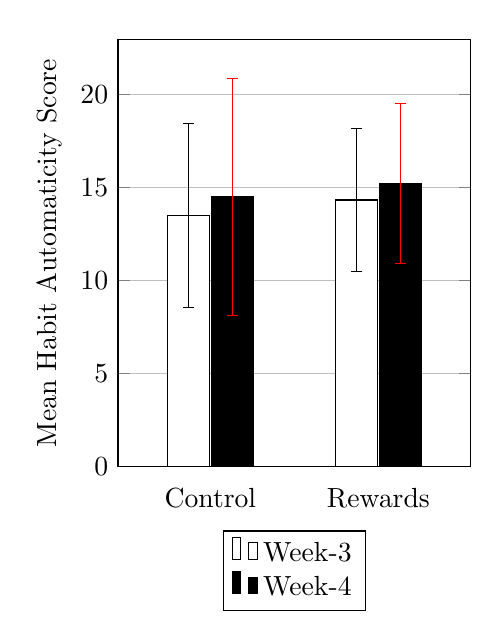
\begin{tikzpicture}
   \begin{axis}[
      width  = 0.5*\textwidth,
      height = 7cm,
      major x tick style = transparent,
      ybar=2*\pgflinewidth,
      bar width=15pt,
      ymajorgrids = true,
      symbolic x coords={Control,Rewards},
      xtick = data,
      scaled y ticks = false,
      enlarge x limits=0.55,
      ymin=0,
      legend cell align=left,
      legend style={at={(0.5,-0.15)},anchor=north},
%       x label style={at={(axis description cs:0.5,-0.1)},anchor=north},
%       y label style={at={(axis description cs:-0.1,.5)},rotate=90,anchor=south},
%       xlabel={$u$ unemployment},
      ylabel={Mean Habit Automaticity Score},
   ]
      \addplot[style={fill=white},error bars/.cd, y dir=both, y explicit]
          coordinates {
          (Control, 13.5) += (0,4.94) -= (0,4.94)
          (Rewards, 14.33) += (0,3.84) -= (0,3.84)
          };

      \addplot[style={fill=black},error bars/.cd, y dir=both, y explicit,error bar style=red]
           coordinates {
           (Control, 14.5) += (0,6.36) -= (0,6.36)
           (Rewards, 15.22) += (0,4.29) -= (0,4.29)
           };

      \legend{Week-3, Week-4}

  \end{axis}
  \end{tikzpicture}
  \caption{H1M2: The rewards affect on habit automaticity. Comparing mean habit automaticity for rewards versus control group.}~\label{fig:m2_h1}

%       S1 Mean S2 Mean S1 SD S2 SD
% Visual  14.6  15.8  4.336 3.701
% Auditory  12    11.5  4.243 6.364
% V-A   16    17.5  2.828 3.536

 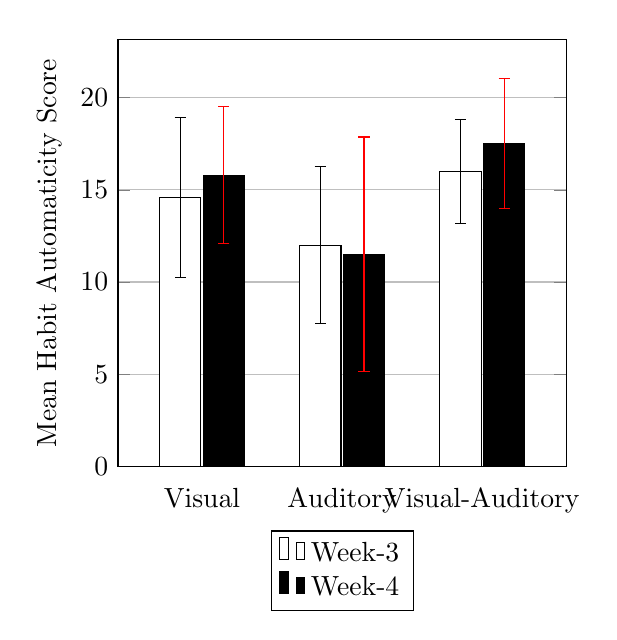
\begin{tikzpicture}
   \begin{axis}[
      width  = 0.6*\textwidth,
      height = 7cm,
      major x tick style = transparent,
      ybar=2*\pgflinewidth,
      bar width=15pt,
      ymajorgrids = true,
      symbolic x coords={Visual,Auditory,Visual-Auditory},
      xtick = data,
      scaled y ticks = false,
      enlarge x limits=0.3, % how far apart the bars are
      ymin=0,
      legend cell align=left,
      legend style={at={(0.5,-0.15)},anchor=north},
%       x label style={at={(axis description cs:0.5,-0.1)},anchor=north},
%       y label style={at={(axis description cs:-0.1,.5)},rotate=90,anchor=south},
%       xlabel={$u$ unemployment},
      ylabel={Mean Habit Automaticity Score},
   ]
      \addplot[style={fill=white},error bars/.cd, y dir=both, y explicit]
          coordinates {
          (Visual, 14.6) += (0,4.336) -= (0,4.336)
          (Auditory, 12) += (0,4.243) -= (0,4.243)
          (Visual-Auditory, 16) += (0,2.828) -= (0,2.828)
          };

      \addplot[style={fill=black},error bars/.cd, y dir=both, y explicit,error bar style=red]
           coordinates {
          (Visual,15.8) += (0,3.701) -= (0,3.701)
          (Auditory, 11.5) += (0,6.364) -= (0,6.364)
          (Visual-Auditory, 17.5) += (0,3.536) -= (0,3.536)
           };

      \legend{Week-3, Week-4}

  \end{axis}
  \end{tikzpicture}
  \caption{H2M2: Multiple modes versus singular on habit performance. Comparing mean habit automaticity for each group.}~\label{fig:m2_h2}
\end{figure}


\subsubsection*{H1M2: the rewards affect on habit automaticity}
An independent-samples t-test was conducted to compare the habit automaticity scores
for rewards and control at both SRBAI 1 and SRBAI 2 (Figure~\ref{fig:m2_h1}). For SRBAI 1, there was also no significant differences in scores for rewards (mean = 14.33, SD = 3.84) and control (mean = 13.50, SD = 4.94; t (9) = 0.224, p = .85,
two-tailed). The magnitude of the differences in the means (mean difference = .83,
95\% CI: \-29.43 to 27.76) was very small (eta squared = .005). For SRBAI 2, there was no significant difference in scores for rewards
(mean = 15.22, SD = 4.29) and control (mean = 14.50, SD = 6.36; t (9) = 0.202, p = .84,
two-tailed). The magnitude of the differences in the means (mean difference = .72,
95\% CI: \-8.80 to 7.36) was very small (eta squared = .004).


A one-way between-groups analysis of variance with planned comparisons was also conducted to explore the impact of rewards on habit automaticity, as measured by the SRBAI 1 and 2. Participants were divided into two groups (Group 1: visual rewards, auditory rewards, visual-auditory rewards combined; Group 2: control group. There was not a
statistically significant difference for the two groups at SRBAI 1: F (1, 9) = 0.02, p = .88, and SRBAI 2: F (1, 9) = 0.07, p = .78. In addition, the difference in mean scores between the groups had, at SRBAI 1: a medium effect with an effect size of .11, and at SRBAI 2: a large effect, with an effect size of .17, both calculated using eta squared.

\subsubsection*{H2M2: multiple modes versus singular mode on habit automaticity}
A one-way between-groups analysis of variance with planned comparisons was conducted to explore the
impact of multiple modalities on habit automaticity, compared with singular modes as measured by the SRBAI 1 and 2 (Figure~\ref{fig:m2_h2}). Participants were divided into two groups according to their reward mode (Group 1: visual rewards, auditory rewards; Group 2: visual-auditory combined rewards). There was not a
statistically significant difference for the two groups at SRBAI 1: F (1, 9) = 1.04, p = .33, and SRBAI 2: F (1, 9) = 0.64, p = .44. In addition, the difference in mean scores between the groups had, at SRBAI 1: a medium effect with an effect size of .11, and at SRBAI 2: a large effect, with an effect size of .17, both calculated using eta squared.



\subsubsection{Interview Feedback}
The interview transcripts were analysed and participants were anonymised following a thematic approach~\cite{thematic_analysis_qualatitive_data}. Below, we consider the role of each participants during the process of interacting with the chatbot and reflect how their interaction may of had a meaningful impact to their formation of a new habit.

\subsubsection*{Questions}

7 interviews with participants outlined their experience with their habit performance after the prototype bot was removed. Participants picked habits they wanted to perform, but when the bot stopped notifying them, they lacked motivation to completed their habit. Some participants enjoyed the rewards at the beginning, but most participants disliked them after the first week.

\begin{itemize}
  \item ``General questions about rewards''
  \item ``Habit formation insight''
  \item ``Chabot interaction''
  \item ``Modality interaction''
  \item ``Are you still doing that habit?''
  \item ``Why did you pick that habit?''
  \item ``Do you want it back?''
\end{itemize}


Participants discussed how they picked their habit, they chose because they had wanted to start for the particular habit for a long time, it was \textit{'not too much effort'} and \textit{'something successful people do'}. They wanted \textit{'to be more active'}, \textit{'relieve stress'} and wanted a habit that was \textit{'less time consuming'}. Throughout, participants mostly completed their habits, but, some participants would put the message off and eventually get their performance would get \textit{'worse and worse'}, until they stopped all together. However, after the bot was removed all interviewed participants (N = 7) found it difficult to continue with their habit. They \textit{'kept forgetting'}, found it \textit{'harder to remember'} and lacked motivation, not performing the action if it had \textit{'been a long day'}. Some tried to do it \textit{'every now and again'}, but usually they would only complete it if \textit{'they remembered'}. This reveals the dependency between technology and habits, suggesting that the bot did not increase habit automaticity, or that the existing routine participants chose was not suitable for new habits, or that they were not given enough time to develop automaticity.


Participants had mixed feelings about the rewards. Some \textit{'did not like the [visual] rewards'}, skipping over them after the first few, they \textit{'just wanted to get rid of the notification dot'}. Another participant said \textit{'some of them [visual-auditory rewards] were funny'}, but they did not like them overall and mentioned the auditory rewards were \textit{'too random'}. One participant thought they did not give them an incentive towards their habit, just a \textit{'nice little extra'}. They also discussed including time-sensitive rewards, as they did not want to listen to music before going to bed. This shows the importance of using an appropriate modality at particular times, e.g. not having auditory rewards at certain times of the day. Finally, an upbeat participant talked about \textit{'always wanting to open them'} and \textit{'the combination was perfect'}. However, they said they also found them \textit{'repetitive'}.


Participants were asked about how they found the chatbot as the method of interaction. They found the method \textit{'pretty good'}, they \textit{'liked it'} and \textit{'would have liked more interaction'}. Suggesting additional features, such as \textit{'help and support throughout'}, \textit{'ideas on how to improve your habit'} and \textit{'advice on how to set aside time for your habit'}. Others were neutral, some expecting \textit{'different messages, such as Hey [name], a bit more care about the person, a bit less like a robot'}. Lots of participants (N = 4) enjoyed the reminder aspect, but a few found it \textit{'repetitive'} and \textit{'got annoying if I pressed Not Yet'}. Participants wanted to see their progress as they tracked their habits, they talked about wanting to reflect on their data. They mentioned that they would feel \textit{'more encouraged to keep doing it, rather than random music [auditory rewards]'}.


Mostly participants wanted the prototype to come back with a few modifications: \textit{'enclosed with Fitbit so it is all in a single place'}, \textit{'fine without rewards'} (2 participants mentioned this), \textit{'more interaction'} and \textit{'with statistics about my progress'}. Participants wanted the bot as more of a \textit{'constant persistent reminder'} with additional tracking elements to remind them to perform their habit to fit into their busy schedule. Participants (N = 5) mentioned the \textit{headspace} app (\url{www.headspace.com}), mentioning that they wanted a combination of the bot and headspace. It prompted another participant to download the headspace app. They wanted the bot to keep on track of their habit and they would use the headspace app to help them perform their mindfulness.  In addition, to interview feedback, two reviews were publicly left on the bot. They echoed interviewees feelings towards the bot.

Review 1: (Rated 2 out of 5) \textit{'I felt a bit like I was being nagged, and I don't like being nagged. The rewards were a bit odd. Would be nice to actually set a time to be asked about the habit.'}


Review 2: (Rated 4 out of 5) \textit{'Interesting project but I did not ultimately feel motivated, the reminders became more of a chore than something I wanted to do.'}


\subsection{Discussion}
This research aimed to understand more about rewards from different modalities and their role in habit formation. Participants receiving bot-delivered rewards completed more habits than the control group without rewards. There was a significant correlation between the habit formation method and habit automaticity. However, this was contradicted during participant interviews (N = 7) where all participants found a drop in habit performance after 1-week without the prototype. Interview discussion and results compare the two hypotheses with each measurement below.

7 interviews with participants outlined their experience with their habit performance after the prototype bot was removed. Participants picked habits they wanted to perform, but when the bot stopped notifying them, they lacked motivation to completed their habit. Some participants enjoyed the rewards at the beginning, but most participants disliked them after the first week.

\subsubsection{Habit Performance}
The results found that participants are more likely to complete their habit if given one of the rewards and participants completed more habits with visual or auditory rewards than visual-auditory rewards.

\subsubsection*{M1H1: The Rewards affect on Habit Performance}
There was a statistically significant drop in habit performance for the control group without rewards. This reveals the effect the rewards had on participant interaction with the bot and habit performance. Although this is contradicted from the interviews where participants discussed negative feelings towards rewards later in the 3-week period. The findings show that rewards did improve habit performance.

\subsubsection*{M1H2: Multiple Modalities affect on Habit Performance}
There is a significant difference between the visual-auditory modes on the number of completed habits. But the result appears to be different to the initial hypotheses, with more participants completing habits with singular mode rewards than multiple. This contradicts the belief that multiple modalities benefits task completion, however these results only impact the particular rewards delivered by this bot. Therefore, it is inconclusive whether multiple modalities rewards in the general sense impact habit performance.


\subsubsection{Habit Automaticity}
It is inconclusive whether the rewards or the combined modalities affected habit automaticity.

\subsubsection*{M2H1: The Rewards affect on Habit Automaticity}
Each individual reward did not have a significant affect on habit automaticity. Although participants with rewards had slightly higher automaticity scores, follow up interviews suggest that automaticity did not develop.

\subsubsection*{M2H2: Multiple Modalities affect on Habit Automaticity}
Participants with visual-auditory combined reward had higher habit automaticity scores compared with visual or auditory rewards. However, these were not statistically significant.


% Under half the participants completed the modality survey (N = 12, 40\%). These had the following rewards: visual rewards had the highest score (the higher, the more participants preferred the reward) (mean = 12, SD = 3.347), visual and auditory rewards were slightly below (mean = 10.75, SD = 1.893).
% TODO: Compare these results to people not using the chatbot, e.g.. people signing up to the gym, new years resolution

\subsubsection{Prototype Success}
The prototype was somewhat successful at running a research trail. There were several issues and various limitations with development. However, it was generally liked by participants and managed to easily gather a lot of useful data.

Participants had mixed feelings towards the bot. Their performance shows that the number of snoozes over time decreased, but the number of total habits completed per day also decreased for all reward types (including the control group). However, participant streaks over time increased and 36 participants manage to use it for 3-weeks.

Participants had various issues with bot interaction. 7 participants tried to message the bot during setup, instead of using the built in \textit{quick reply} buttons. This broke the setup flow and they had to start again. Other participants tried to send multiple messages when asked for free input, they went around an endless loop when asking for a habit type and participants tried to mark their habit as completed using the Facebook Messenger thumb emotion (which the bot was not coded for).

Participants gave additional feedback by simply messaging the bot. They asked inquisitive questions, such as \textit{'what kind of thing are you looking to find out'}, \textit{'this is not working for me'} and \textit{'stop'}---to try and stop the daily messages (the participant then blocked the bot). Negative feedback towards the rewards and bot were also expressed. When asked about being messaged every day, a participant sent this reply and then blocked the bot: \textit{'Do not do that, it will be annoying'}, and another said \textit{'never message me'}. Another stated that this was the \textit{'lame same band'} after receiving a auditory reward.

Mostly participants chose existing routines that were suggested to them. For example, during the pilot trials when asking for an existing routine, users were confused, so examples of habit contexts were provided. The results found, 31 (84\%) participants chose one of the contexts that were listed as examples, some with a slight change in before and after wording, e.g. \textit{before} getting home from work, rather than \textit{after} getting home from work. The remaining 5 participants chose the following context: \textit{'Having a snack'}, \textit{'Sitting in bed'}, \textit{'Early morning'}, \textit{'During breakfast'} and \textit{'Before sleeping'}. A participant also pointed out that changing the time their existing routine occurred was prompted to them, but the description about it, was not.

Participants were able to personalise the chatbot with several different variable configurations. This personalisation could have effected the findings by not narrowing the condition variables. Replicating this research with tighter a configuration is needed to validate this line of reasoning.


\subsubsection*{Dependence}
Streaks could have been better used to give insight to participants progress and challenged them to maintain it, using loss aversion~\cite{loss_aversion} to compare the impact of their broken streak with the gain of keeping it. However, all participants interviewed (N = 7) struggled with maintaining habit performance after the bot was removed. This suggests a dependence between the technology and the habit as participants depended on bot notifications to continue repeating the desired action.


